\documentclass[
  shownotes,
  xcolor={svgnames},
  hyperref={colorlinks,citecolor=DarkBlue,linkcolor=DarkRed,urlcolor=DarkBlue}
  , aspectratio=169]{beamer}
\usepackage{animate}
\usepackage{amsmath}
\usepackage{amsfonts}
\usepackage{amssymb}
\usepackage{pifont}
\usepackage{mathpazo}
%\usepackage{xcolor}
\usepackage{multimedia}
\usepackage{fancybox}
\usepackage[para]{threeparttable}
\usepackage{multirow}
\setcounter{MaxMatrixCols}{30}
\usepackage{subcaption}
\usepackage{graphicx}
\usepackage{lscape}
\usepackage[compatibility=false,font=small]{caption}
\usepackage{booktabs}
\usepackage{ragged2e}
\usepackage{chronosys}
\usepackage{appendixnumberbeamer}
\usepackage{animate}
\setbeamertemplate{caption}[numbered]
\usepackage{color}
%\usepackage{times}
\usepackage{tikz}
\usepackage{comment} %to comment
%% BibTeX settings
\usepackage{natbib}
\bibliographystyle{apalike}
\bibpunct{(}{)}{,}{a}{,}{,}
\setbeamertemplate{bibliography item}{[\theenumiv]}

% Defines columns for bespoke tables
\usepackage{array}
\newcolumntype{L}[1]{>{\raggedright\let\newline\\\arraybackslash\hspace{0pt}}m{#1}}
\newcolumntype{C}[1]{>{\centering\let\newline\\\arraybackslash\hspace{0pt}}m{#1}}
\newcolumntype{R}[1]{>{\raggedleft\let\newline\\\arraybackslash\hspace{0pt}}m{#1}}


\usepackage{xfrac}


\usepackage{multicol}
\setlength{\columnsep}{0.5cm}

% Theme and colors
\usetheme{Boadilla}

% I use steel blue and a custom color palette. This defines it.
\definecolor{andesred}{HTML}{af2433}

% Other options
\providecommand{\U}[1]{\protect\rule{.1in}{.1in}}
\usefonttheme{serif}
\setbeamertemplate{itemize items}[default]
\setbeamertemplate{enumerate items}[square]
\setbeamertemplate{section in toc}[circle]

\makeatletter

\definecolor{mybackground}{HTML}{82CAFA}
\definecolor{myforeground}{HTML}{0000A0}

\setbeamercolor{normal text}{fg=black,bg=white}
\setbeamercolor{alerted text}{fg=red}
\setbeamercolor{example text}{fg=black}

\setbeamercolor{background canvas}{fg=myforeground, bg=white}
\setbeamercolor{background}{fg=myforeground, bg=mybackground}

\setbeamercolor{palette primary}{fg=black, bg=gray!30!white}
\setbeamercolor{palette secondary}{fg=black, bg=gray!20!white}
\setbeamercolor{palette tertiary}{fg=white, bg=andesred}

\setbeamercolor{frametitle}{fg=andesred}
\setbeamercolor{title}{fg=andesred}
\setbeamercolor{block title}{fg=andesred}
\setbeamercolor{itemize item}{fg=andesred}
\setbeamercolor{itemize subitem}{fg=andesred}
\setbeamercolor{itemize subsubitem}{fg=andesred}
\setbeamercolor{enumerate item}{fg=andesred}
\setbeamercolor{item projected}{bg=gray!30!white,fg=andesred}
\setbeamercolor{enumerate subitem}{fg=andesred}
\setbeamercolor{section number projected}{bg=gray!30!white,fg=andesred}
\setbeamercolor{section in toc}{fg=andesred}
\setbeamercolor{caption name}{fg=andesred}
\setbeamercolor{button}{bg=gray!30!white,fg=andesred}


\usepackage{fancyvrb}
\newcommand{\VerbBar}{|}
\newcommand{\VERB}{\Verb[commandchars=\\\{\}]}
\DefineVerbatimEnvironment{Highlighting}{Verbatim}{commandchars=\\\{\}}
% Add ',fontsize=\small' for more characters per line
\usepackage{framed}
\definecolor{shadecolor}{RGB}{248,248,248}
\newenvironment{Shaded}{\begin{snugshade}}{\end{snugshade}}
\newcommand{\AlertTok}[1]{\textcolor[rgb]{0.94,0.16,0.16}{#1}}
\newcommand{\AnnotationTok}[1]{\textcolor[rgb]{0.56,0.35,0.01}{\textbf{\textit{#1}}}}
\newcommand{\AttributeTok}[1]{\textcolor[rgb]{0.77,0.63,0.00}{#1}}
\newcommand{\BaseNTok}[1]{\textcolor[rgb]{0.00,0.00,0.81}{#1}}
\newcommand{\BuiltInTok}[1]{#1}
\newcommand{\CharTok}[1]{\textcolor[rgb]{0.31,0.60,0.02}{#1}}
\newcommand{\CommentTok}[1]{\textcolor[rgb]{0.56,0.35,0.01}{\textit{#1}}}
\newcommand{\CommentVarTok}[1]{\textcolor[rgb]{0.56,0.35,0.01}{\textbf{\textit{#1}}}}
\newcommand{\ConstantTok}[1]{\textcolor[rgb]{0.00,0.00,0.00}{#1}}
\newcommand{\ControlFlowTok}[1]{\textcolor[rgb]{0.13,0.29,0.53}{\textbf{#1}}}
\newcommand{\DataTypeTok}[1]{\textcolor[rgb]{0.13,0.29,0.53}{#1}}
\newcommand{\DecValTok}[1]{\textcolor[rgb]{0.00,0.00,0.81}{#1}}
\newcommand{\DocumentationTok}[1]{\textcolor[rgb]{0.56,0.35,0.01}{\textbf{\textit{#1}}}}
\newcommand{\ErrorTok}[1]{\textcolor[rgb]{0.64,0.00,0.00}{\textbf{#1}}}
\newcommand{\ExtensionTok}[1]{#1}
\newcommand{\FloatTok}[1]{\textcolor[rgb]{0.00,0.00,0.81}{#1}}
\newcommand{\FunctionTok}[1]{\textcolor[rgb]{0.00,0.00,0.00}{#1}}
\newcommand{\ImportTok}[1]{#1}
\newcommand{\InformationTok}[1]{\textcolor[rgb]{0.56,0.35,0.01}{\textbf{\textit{#1}}}}
\newcommand{\KeywordTok}[1]{\textcolor[rgb]{0.13,0.29,0.53}{\textbf{#1}}}
\newcommand{\NormalTok}[1]{#1}
\newcommand{\OperatorTok}[1]{\textcolor[rgb]{0.81,0.36,0.00}{\textbf{#1}}}
\newcommand{\OtherTok}[1]{\textcolor[rgb]{0.56,0.35,0.01}{#1}}
\newcommand{\PreprocessorTok}[1]{\textcolor[rgb]{0.56,0.35,0.01}{\textit{#1}}}
\newcommand{\RegionMarkerTok}[1]{#1}
\newcommand{\SpecialCharTok}[1]{\textcolor[rgb]{0.00,0.00,0.00}{#1}}
\newcommand{\SpecialStringTok}[1]{\textcolor[rgb]{0.31,0.60,0.02}{#1}}
\newcommand{\StringTok}[1]{\textcolor[rgb]{0.31,0.60,0.02}{#1}}
\newcommand{\VariableTok}[1]{\textcolor[rgb]{0.00,0.00,0.00}{#1}}
\newcommand{\VerbatimStringTok}[1]{\textcolor[rgb]{0.31,0.60,0.02}{#1}}
\newcommand{\WarningTok}[1]{\textcolor[rgb]{0.56,0.35,0.01}{\textbf{\textit{#1}}}}
\usepackage{graphicx}
\makeatletter

\definecolor{airforceblue}{rgb}{0.36, 0.54, 0.66}

\usepackage{tikz}
% Tikz settings optimized for causal graphs.
\usetikzlibrary{shapes,decorations,arrows,calc,arrows.meta,fit,positioning}
\tikzset{
    -Latex,auto,node distance =1 cm and 1 cm,semithick,
    state/.style ={ellipse, draw, minimum width = 0.7 cm},
    point/.style = {circle, draw, inner sep=0.04cm,fill,node contents={}},
    bidirected/.style={Latex-Latex,dashed},
    el/.style = {inner sep=2pt, align=left, sloped}
}


\makeatother






%%%%%%%%%%%%%%% BEGINS DOCUMENT %%%%%%%%%%%%%%%%%%

\begin{document}
 
\title[Lecture 22]{Lecture 22: \\ Bagging, Random Forests, \& Boosting}
\subtitle{Big Data and Machine Learning for Applied Economics \\ Econ 4676}
\date{\today}

\author[Sarmiento-Barbieri]{Ignacio Sarmiento-Barbieri}
\institute[Uniandes]{Universidad de los Andes}


\begin{frame}[noframenumbering]
\maketitle
\end{frame}

%%%%%%%%%%%%%%%%%%%%%%%%%%%%%%%%%%%




%----------------------------------------------------------------------% 

\begin{frame}
\frametitle{Agenda}

\tableofcontents

\end{frame}
%----------------------------------------------------------------------%
\section{Recap w. Example: Beauty in the classroom }
%----------------------------------------------------------------------%
\begin{frame}[fragile]
\frametitle{CART: Recap w. Example: Beauty in the classroom}




  \begin{figure}[H] \centering
            \captionsetup{justification=centering}
              
\includegraphics[scale=0.4]{figures/beauty_hamermesh}
              
 \end{figure}

\end{frame}

%----------------------------------------------------------------------%
\begin{frame}[fragile]
\frametitle{CART: Recap w. Example: Beauty in the classroom}
\framesubtitle{Motivation}

\begin{itemize}
\item An immense literature in social psychology (summarized by Hatfield and Sprecher, 1986) has  examined  the  impact  of  human  beauty  on  a  variety  of  noneconomic  outcomes.   
\medskip
\item Economists have considered how beauty affects labor market outcomes, particularly earnings (Hamermesh  and  Biddle,  1994;  Biddle  and  Hamermesh,  1998).   
\medskip
\item  The  impacts  on  these  monetary  outcomes are implicitly the end results of the effects of beauty on productivity; 

\item But there seems to be  no  direct  evidence  of  the  impacts  of  beauty  on  productivity  in  a  context  in  which  we  can  be  fairly sure that productivity generates economic rewards. 


\end{itemize}

\end{frame}

%----------------------------------------------------------------------%
\begin{frame}[fragile]
\frametitle{CART: Recap w. Example: Beauty in the classroom}
\framesubtitle{Motivation}


\begin{itemize}
  \item A substantial amount of research has indicated that academic administrators pay attention to teaching quality in setting salaries (Becker and Watts, 1999). 
  \medskip
  \item  The question  is  what  generates  the  measured  productivity  for  which  the  economic  rewards  are  being  offered.  
  \medskip
\item One possibility is simply that descriptive characteristics, such as beauty, trigger positive responses  by  students  and  lead  them  to  evaluate  some  teachers  more  favorably,  so  that  their  beauty earns them higher economic returns. 


\end{itemize}

\end{frame}

%----------------------------------------------------------------------%
\begin{frame}[fragile]
\frametitle{CART: Recap w. Example: Beauty in the classroom}
\framesubtitle{Motivation}


\begin{itemize}
\item They take sample of student instructional ratings for a group of university teachers and acquire six independent measures of their beauty, and a number of other descriptors of them and their classes. 
\end{itemize}


\begin{scriptsize}
\begin{Shaded}
\begin{Highlighting}[]
\KeywordTok{data}\NormalTok{(}\StringTok{"TeachingRatings"}\NormalTok{, }\DataTypeTok{package =} \StringTok{"AER"}\NormalTok{)}
\NormalTok{tr \textless{}{-}}\StringTok{ }\KeywordTok{subset}\NormalTok{(TeachingRatings, credits }\OperatorTok{==}\StringTok{ "more"}\NormalTok{)}
\KeywordTok{str}\NormalTok{(tr)}
\end{Highlighting}
\end{Shaded}

\end{scriptsize}
\begin{tiny}

\begin{verbatim}
## 'data.frame':    436 obs. of  12 variables:
##  $ minority   : Factor w/ 2 levels "no","yes": 2 1 1 1 1 1 1 1 1 1 ...
##  $ age        : int  36 59 51 40 31 62 33 51 33 47 ...
##  $ gender     : Factor w/ 2 levels "male","female": 2 1 1 2 2 1 2 2 2 1 ...
##  $ credits    : Factor w/ 2 levels "more","single": 1 1 1 1 1 1 1 1 1 1 ...
##  $ beauty     : num  0.29 -0.738 -0.572 -0.678 1.51 ...
##  $ eval       : num  4.3 4.5 3.7 4.3 4.4 4.2 4 3.4 4.5 3.9 ...
##  $ division   : Factor w/ 2 levels "upper","lower": 1 1 1 1 1 1 1 1 1 1 ...
##  $ native     : Factor w/ 2 levels "yes","no": 1 1 1 1 1 1 1 1 1 1 ...
##  $ tenure     : Factor w/ 2 levels "no","yes": 2 2 2 2 2 2 2 2 2 1 ...
##  $ students   : num  24 17 55 40 42 182 33 25 48 16 ...
##  $ allstudents: num  43 20 55 46 48 282 41 41 60 19 ...
##  $ prof       : Factor w/ 94 levels "1","2","3","4",..: 1 2 3 4 5 6 7 8 9 10 ...
\end{verbatim}


\end{tiny}   
\end{frame}

%----------------------------------------------------------------------%
\begin{frame}[fragile]
\frametitle{CART: Recap w. Example: Beauty in the classroom}
\framesubtitle{OLS}

\begin{scriptsize}
\begin{Shaded}
\begin{Highlighting}[]
\NormalTok{tr\_lm \textless{}{-}}\StringTok{ }\KeywordTok{lm}\NormalTok{(eval }\OperatorTok{\textasciitilde{}}\StringTok{ }\NormalTok{beauty }\OperatorTok{+}\StringTok{ }\NormalTok{gender }\OperatorTok{+}\StringTok{ }\NormalTok{minority }\OperatorTok{+}\StringTok{ }\NormalTok{native }\OperatorTok{+}\StringTok{ }\NormalTok{tenure }\OperatorTok{+}\StringTok{ }\NormalTok{division,}
  \DataTypeTok{data =}\NormalTok{ tr, }\DataTypeTok{weights =}\NormalTok{ students)}

\NormalTok{tr\_lm\_gender \textless{}{-}}\StringTok{ }\KeywordTok{lm}\NormalTok{(eval }\OperatorTok{\textasciitilde{}}\StringTok{ }\NormalTok{beauty}\OperatorTok{:}\NormalTok{gender }\OperatorTok{+}\StringTok{ }\NormalTok{minority }\OperatorTok{+}\StringTok{ }\NormalTok{native }\OperatorTok{+}\StringTok{ }\NormalTok{tenure }\OperatorTok{+}\StringTok{ }\NormalTok{division,}
  \DataTypeTok{data =}\NormalTok{ tr, }\DataTypeTok{weights =}\NormalTok{ students)}

\NormalTok{tr\_lm\_male \textless{}{-}}\StringTok{ }\KeywordTok{lm}\NormalTok{(eval }\OperatorTok{\textasciitilde{}}\StringTok{ }\NormalTok{beauty }\OperatorTok{+}\StringTok{ }\NormalTok{minority }\OperatorTok{+}\StringTok{ }\NormalTok{native }\OperatorTok{+}\StringTok{ }\NormalTok{tenure }\OperatorTok{+}\StringTok{ }\NormalTok{division,}
  \DataTypeTok{data =}\NormalTok{ tr[tr}\OperatorTok{$}\NormalTok{gender}\OperatorTok{==}\StringTok{"male"}\NormalTok{,], }\DataTypeTok{weights =}\NormalTok{ students)}

\NormalTok{tr\_lm\_female \textless{}{-}}\StringTok{ }\KeywordTok{lm}\NormalTok{(eval }\OperatorTok{\textasciitilde{}}\StringTok{ }\NormalTok{beauty }\OperatorTok{+}\StringTok{ }\NormalTok{minority }\OperatorTok{+}\StringTok{ }\NormalTok{native }\OperatorTok{+}\StringTok{ }\NormalTok{tenure }\OperatorTok{+}\StringTok{ }\NormalTok{division,}
  \DataTypeTok{data =}\NormalTok{ tr[tr}\OperatorTok{$}\NormalTok{gender}\OperatorTok{==}\StringTok{"female"}\NormalTok{,], }\DataTypeTok{weights =}\NormalTok{ students)}

\NormalTok{stargazer}\OperatorTok{::}\KeywordTok{stargazer}\NormalTok{(tr\_lm,tr\_lm\_gender,tr\_lm\_male,tr\_lm\_female,}\DataTypeTok{type=}\StringTok{"text"}\NormalTok{)}
\end{Highlighting}
\end{Shaded}
\end{scriptsize}

\end{frame}
%----------------------------------------------------------------------%
\begin{frame}[fragile]
\frametitle{CART: Recap w. Example: Beauty in the classroom}
\framesubtitle{OLS}


\begin{tiny}
\begin{verbatim}
## ==================================================================================================================
##                                                          Dependent variable:                                      
##                     ----------------------------------------------------------------------------------------------
##                                                                  eval                                             
##                               (1)                     (2)                     (3)                    (4)          
## ------------------------------------------------------------------------------------------------------------------
## beauty                     0.283***                                        0.383***                0.133***       
##                             (0.028)                                         (0.037)                (0.045)        
## genderfemale               -0.213***                                                                              
##                             (0.048)                                                                               
## minorityyes                -0.327***               -0.363***                -0.014                -0.279***       
##                             (0.086)                 (0.084)                 (0.194)                (0.098)        
## nativeno                    -0.217*                 -0.229*                -0.388**                 -0.288        
##                             (0.125)                 (0.124)                 (0.188)                (0.175)        
## tenureyes                  -0.132**                 -0.032                  -0.053                  -0.064        
##                             (0.065)                 (0.065)                 (0.088)                (0.098)        
## divisionlower               -0.050                  -0.071                   0.004                -0.244***       
##                             (0.044)                 (0.045)                 (0.054)                (0.078)        
## beauty:gendermale                                  0.407***                                                       
##                                                     (0.038)                                                       
## beauty:genderfemale                                0.132***                                                       
##                                                     (0.043)                                                       
## Constant                   4.216***                4.058***                4.101***                4.027***       
##                             (0.068)                 (0.062)                 (0.089)                (0.084)        
##                                                                                                                   
## ------------------------------------------------------------------------------------------------------------------
## Observations                  436                     436                     250                    186          
## R2                           0.271                   0.275                   0.335                  0.170         
## ==================================================================================================================
## Note:                                                                                  *p<0.1; **p<0.05; ***p<0.01
\end{verbatim}




\end{tiny}


\end{frame}
%----------------------------------------------------------------------%
\begin{frame}[fragile]
\frametitle{CART: Recap w. Example: Beauty in the classroom}
\framesubtitle{Trees}

\begin{scriptsize}
\begin{Shaded}
\begin{Highlighting}[]
\KeywordTok{library}\NormalTok{(}\StringTok{"tree"}\NormalTok{)}

\NormalTok{pstree \textless{}{-}}\StringTok{ }\KeywordTok{tree}\NormalTok{(eval }\OperatorTok{\textasciitilde{}}\NormalTok{beauty }\OperatorTok{+}\StringTok{ }\NormalTok{gender }\OperatorTok{+}\StringTok{ }\NormalTok{minority }\OperatorTok{+}\StringTok{ }\NormalTok{native }\OperatorTok{+}\StringTok{ }\NormalTok{tenure }\OperatorTok{+}\StringTok{ }\NormalTok{division, }\DataTypeTok{data=}\NormalTok{tr, }\DataTypeTok{mincut=}\DecValTok{1}\NormalTok{)}
\KeywordTok{par}\NormalTok{(}\DataTypeTok{mfrow=}\KeywordTok{c}\NormalTok{(}\DecValTok{1}\NormalTok{,}\DecValTok{1}\NormalTok{))}
\KeywordTok{plot}\NormalTok{(pstree, }\DataTypeTok{col=}\DecValTok{8}\NormalTok{)}
\KeywordTok{text}\NormalTok{(pstree, }\DataTypeTok{digits=}\DecValTok{2}\NormalTok{)}
\end{Highlighting}
\end{Shaded}
\end{scriptsize}

\begin{figure}[H] \centering
            \captionsetup{justification=centering}
              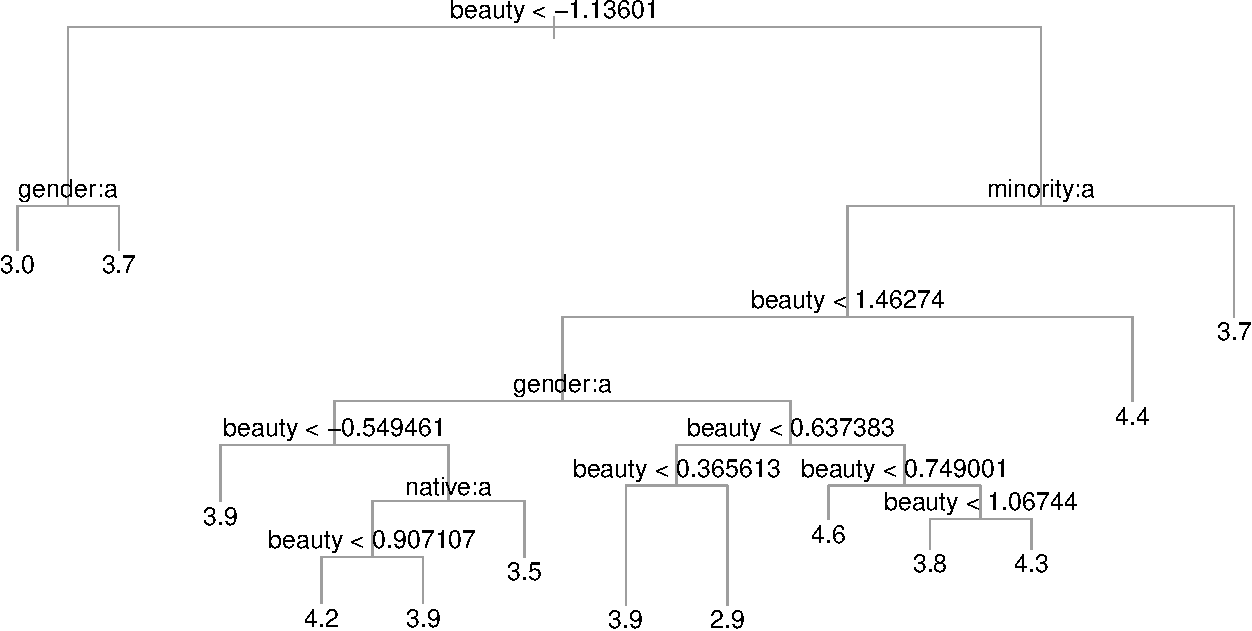
\includegraphics[scale=0.4]{figures/unnamed-chunk-3-1.pdf}              
 \end{figure}

\end{frame}

%----------------------------------------------------------------------%
\begin{frame}[fragile]
\frametitle{CART: Recap w. Example: Beauty in the classroom}
\framesubtitle{Trees: Constructing the partition}


\begin{itemize}
 \item How to choose the partition?
 \item Start with the trivial partition with one element
 \item  Greedy algorithm (CART): Iteratively split an element of the partition, such that the in-sample prediction improves as much as possible.
 \item That is: Given $(R_1\dots,R_M)$
 \begin{itemize}
  \item For each $R_m$ $m=1,\dots,M$ and
  \item For each $X_j$ $j=1,\dots,p$
  \item find the $s_{j,m}$ that minimizes the mean squared error, if we split $R_m$ along variable $X_j$ at $s_{j,m}$
  \item then pick the $(m,j)$ that minimizes the MSE and construct a new partition with $M+1$ elements
  \item Iterate
 \end{itemize}
 
\end{itemize}
\end{frame}

%----------------------------------------------------------------------%
\begin{frame}[fragile]
\frametitle{CART: Recap w. Example: Beauty in the classroom}
\framesubtitle{Trees: Tuning and pruning}

\begin{itemize}
\item Key tuning parameter: Total number of splits M.
\item We can optimize this via cross-validation.
\item CART can furthermore be improved using “pruning.”
\item Idea:
\begin{itemize}
\item Fit a flexible tree (with large M) using CART.
\item Then iteratively remove (collapse) nodes.
\item To minimize the sum of squared errors,
\item plus a penalty for the number of elements in the partition.
\end{itemize}

\item This improves upon greedy search. It yields smaller trees for the same mean squared error.
\end{itemize}

\end{frame}
%----------------------------------------------------------------------%
\begin{frame}[fragile]
\frametitle{CART: Recap w. Example: Beauty in the classroom}
\framesubtitle{Trees}

\begin{scriptsize}
\begin{Shaded}
\begin{Highlighting}[]
\CommentTok{\#\# Use cross{-}validation to prune the tree}
\NormalTok{cvpst \textless{}{-}}\StringTok{ }\KeywordTok{cv.tree}\NormalTok{(pstree, }\DataTypeTok{K=}\DecValTok{10}\NormalTok{)}
\KeywordTok{plot}\NormalTok{(cvpst}\OperatorTok{$}\NormalTok{size, cvpst}\OperatorTok{$}\NormalTok{dev, }\DataTypeTok{xlab=}\StringTok{"size"}\NormalTok{, }\DataTypeTok{ylab=}\StringTok{"oos deviance"}\NormalTok{, }\DataTypeTok{pch=}\DecValTok{21}\NormalTok{, }\DataTypeTok{bg=}\StringTok{"lightblue"}\NormalTok{, }\DataTypeTok{bty=}\StringTok{"n"}\NormalTok{)}
\end{Highlighting}
\end{Shaded}
\end{scriptsize}

\begin{figure}[H] \centering
            \captionsetup{justification=centering}
              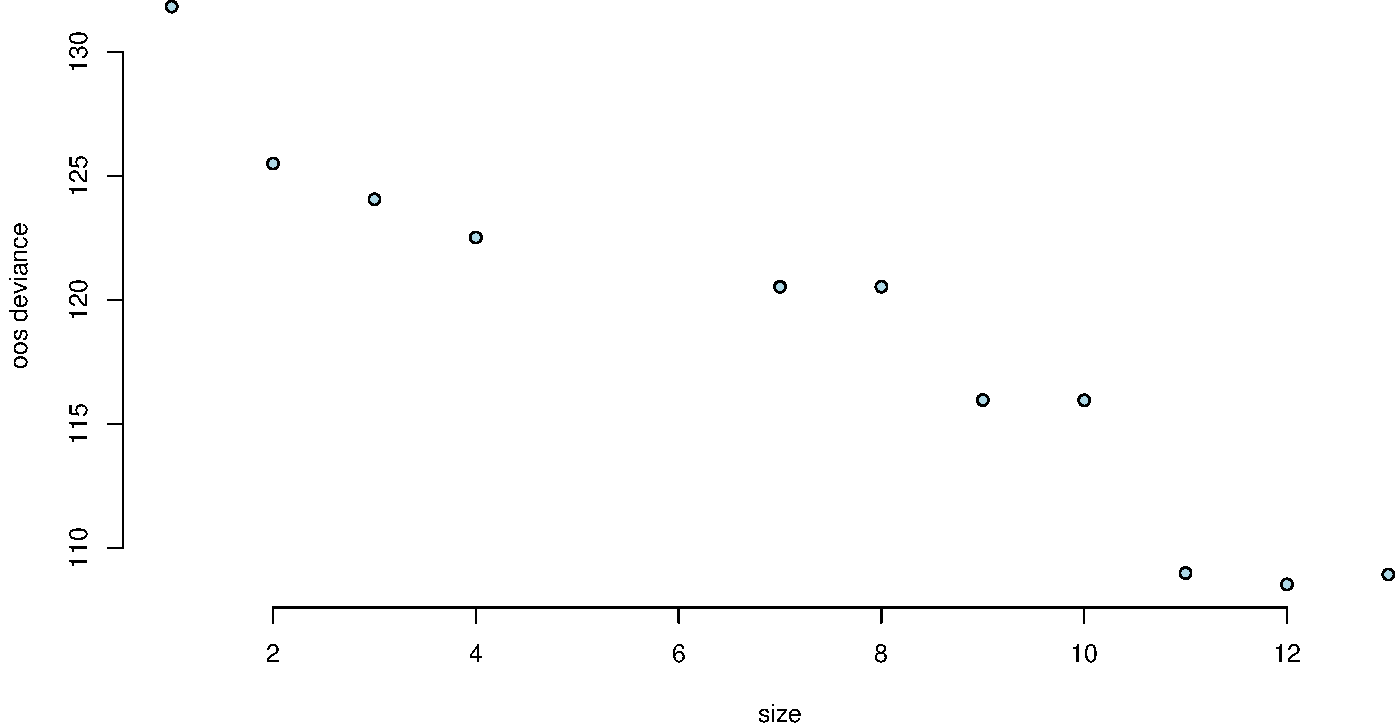
\includegraphics[scale=0.4]{figures/unnamed-chunk-4-1.pdf}              
 \end{figure}

\end{frame}
%----------------------------------------------------------------------%
\begin{frame}[fragile]
\frametitle{CART: Recap w. Example: Beauty in the classroom}
\framesubtitle{Trees}

\begin{scriptsize}
\begin{Shaded}
\begin{Highlighting}[]
\NormalTok{pstcut \textless{}{-}}\StringTok{ }\KeywordTok{prune.tree}\NormalTok{(pstree, }\DataTypeTok{best=}\DecValTok{12}\NormalTok{)}
\KeywordTok{plot}\NormalTok{(pstcut, }\DataTypeTok{col=}\DecValTok{8}\NormalTok{)}
\KeywordTok{text}\NormalTok{(pstcut)}
\end{Highlighting}
\end{Shaded}

\end{scriptsize}
\begin{figure}[H] \centering
            \captionsetup{justification=centering}
              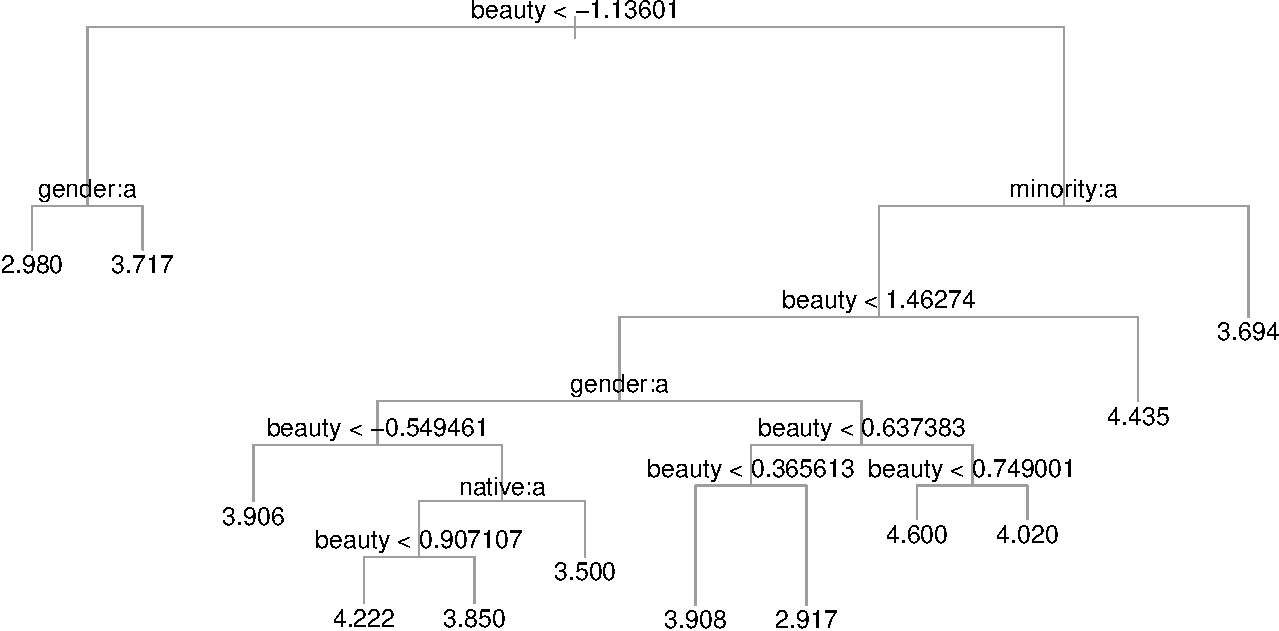
\includegraphics[scale=0.4]{figures/unnamed-chunk-6-1.pdf}              
 \end{figure}


\end{frame}

%----------------------------------------------------------------------%
\begin{frame}[fragile]
\frametitle{CARTs}

\begin{itemize}
  \item Smart way to represent nonlinearities. Most relevant variables on top.
  \medskip
  \item Very easy to communicate.
  \medskip
  \item  Reproduces human decision-making process.
  \medskip
  \item Trees are intuitive and do OK, but
  \begin{itemize}
    \item They are not very good at prediction 
  \item If the structure is linear, CART does not work well.
  \item  Not very robust
  \end{itemize}
  
\end{itemize}



\end{frame}
%----------------------------------------------------------------------%
\section{Bagging and Random Forests }
%----------------------------------------------------------------------%
\begin{frame}[fragile]
\frametitle{Bagging}

\begin{itemize}
  \item Problem with CART: high variance.
  \item We can improve performance a lot using either bootstrap aggregation (bagging), random forests, or boosting.
  \item Bagging:
    \begin{itemize}
      \item Repeatedly draw bootstrap samples $(X_i^b,Y_i^b)_{i=1}^N$ from the observed sample.
      \item For each bootstrap sample, fit a regression tree $\hat{f}^b(x)$
      \item Average across bootstrap samples to get the predictor
      \begin{align}
        \hat{f}_{bag} =\frac{1}{B}\sum_{b=1}^B \hat{f}^b(x)
      \end{align}
\item Basically we are smoothing predictions. 
\item Idea: the variance of the average is less than that of a single prediction.
\end{itemize}

\end{itemize}

\end{frame}

%----------------------------------------------------------------------%
\begin{frame}[fragile]
\frametitle{Random Forests}

\begin{itemize}
\item Problem with bagging: if there is a strong predictor, different trees are very similar to each other. High correlation. Is the variance really reduced?
\bigskip
\item Forests: lower the correlation between the trees in the boostrap.
\bigskip
\item If there are $p$ predictors, in each partition use only $m <p$ predictors, chosen randomly
\bigskip
\item Bagging is forest with $m = p$ (use all predictors in each partition).
\bigskip
\item Typically $m = \sqrt(p)$
\end{itemize}

\end{frame}
%----------------------------------------------------------------------%
\begin{frame}[fragile]
\frametitle{Random Forests}

\begin{figure}[H] \centering
            \captionsetup{justification=centering}
              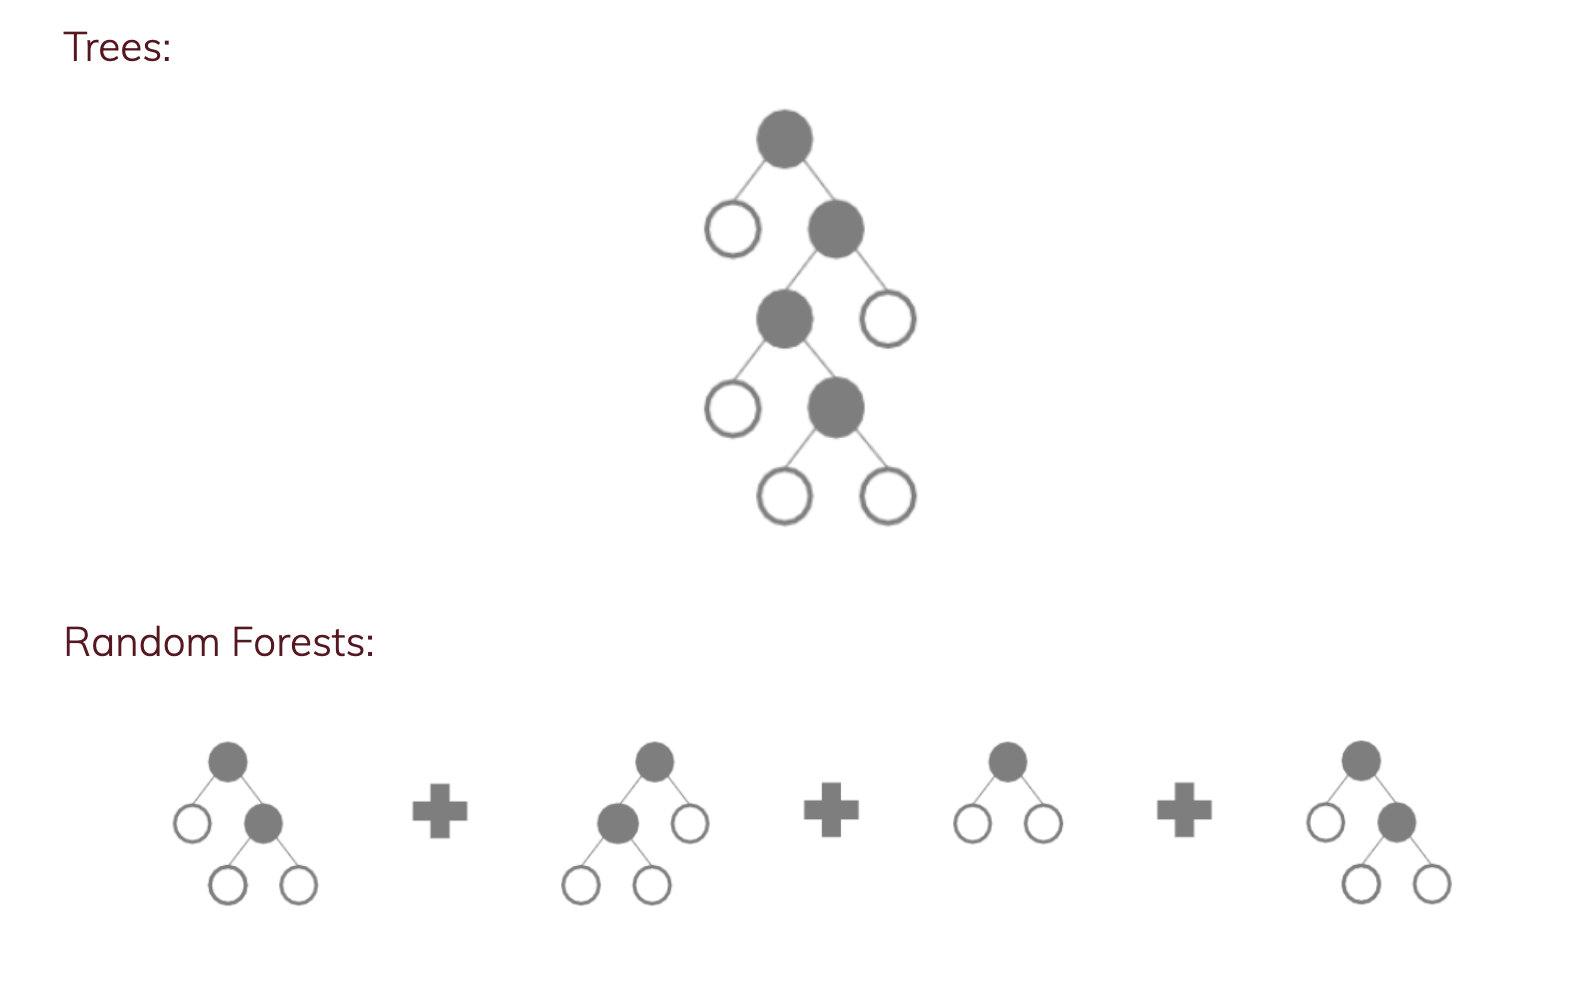
\includegraphics[scale=0.4]{figures/trees_to_forests.png}
 \end{figure}
\end{frame}

%----------------------------------------------------------------------%
\begin{frame}[fragile]
\frametitle{Random Forests}

\begin{Shaded}
\begin{Highlighting}[]
\KeywordTok{require}\NormalTok{(}\StringTok{"ranger"}\NormalTok{)}

\NormalTok{rf\_tree \textless{}{-}}\StringTok{ }\KeywordTok{ranger}\NormalTok{(eval }\OperatorTok{\textasciitilde{}}\NormalTok{beauty }\OperatorTok{+}\StringTok{ }\NormalTok{gender }\OperatorTok{+}\StringTok{ }\NormalTok{minority }\OperatorTok{+}\StringTok{ }\NormalTok{native }\OperatorTok{+}
        \StringTok{ }\NormalTok{tenure }\OperatorTok{+}\StringTok{ }\NormalTok{division, }\DataTypeTok{data=}\NormalTok{tr, }
        \DataTypeTok{write.forest=}\OtherTok{TRUE}\NormalTok{,}\DataTypeTok{num.tree=}\DecValTok{200}\NormalTok{,}\DataTypeTok{min.node.size=}\DecValTok{25}\NormalTok{,}
        \DataTypeTok{importance=}\StringTok{"impurity"}\NormalTok{)}
\KeywordTok{sort}\NormalTok{(rf\_tree}\OperatorTok{$}\NormalTok{variable.importance, }\DataTypeTok{decreasing =} \OtherTok{TRUE}\NormalTok{)}
\end{Highlighting}
\end{Shaded}

\begin{verbatim}
##    beauty  minority    gender    native    tenure  division 
## 22.881176  3.089366  2.608295  2.104095  2.062075  1.627261
\end{verbatim}

\end{frame}
%----------------------------------------------------------------------%
\section{Boosting}
%----------------------------------------------------------------------%
\begin{frame}[fragile]
\frametitle{Boosting}

\begin{itemize}
\item Problem with CART: high variance. Instability
\medskip
\item Weak classifier: marginally better classifier than flipping a coin (error rate slightly better than .5)
\medskip
\item E.g.: CART with few branches ('stump', two branches)
\medskip
\item Boosting: weighted average of a succession of weak classifiers.
\medskip
\item Vocab
\medskip
  \begin{itemize}
  \item $y \in {-1,1}$ (for simplicity), $X$ vector of predictors.
  \medskip
  \item $y = G (X)$ (classifier)
  \medskip
  \item $err = \frac{1}{N} \sum_{i}^N I(y_i\neq G(x_i))$
  \end{itemize}
\end{itemize}


\end{frame}

%----------------------------------------------------------------------%
\subsection{AdaBoost}
%----------------------------------------------------------------------%
\begin{frame}[fragile]
\frametitle{AdaBoost}
\begin{enumerate}
\item Start with weights $w_i = 1 / N$
\item For m = 1 through M:
\begin{enumerate}
    \item Adjust $G_m(x)$ using weights $w_i$ .
    \item Compute prediction 
    \begin{align}
    err_m = \frac{\sum_{i=1}^N  I(y_i \neq G_m(x_i))}{\sum_{i=1}^N w_i}
    \end{align}
    \item Compute $\alpha_m= ln \left[\frac{(1 - err m )}{ err m} \right]$
    \item Update weights: $w_i \leftarrow w_i c_i$ 
    \begin{align}
    c_i = exp \left[\alpha_m  I (y i \neq G_m (x_i )) \right]
    \end{align}
    
\end{enumerate}
\item Output: $G(x) = sgn[\sum_{m = 1}^M \alpha_m G_m(x)]$
\end{enumerate}

\end{frame} 
%----------------------------------------------------------------------%
\begin{frame}[fragile]
\frametitle{AdaBoost}

\begin{itemize}
\item $c_i = exp \left[ \alpha_m I(y_i \neq G_m (x_i )) \right]$
\medskip
\item If it was correctly predicted, $c_i = 1$. No issue.
\medskip
\item Otherwise, $c_i = exp (\alpha_m ) = \frac{(1 - err_m ) }{err_m} > 1$ 
\medskip
\item At each step the method gives more relative importance to the predictions that where wrong.
\medskip
\item Final step: weighted average of predictions at each step.
\end{itemize}
\end{frame}
%----------------------------------------------------------------------%
\begin{frame}[fragile]
\frametitle{AdaBoost}


\begin{figure}[H] \centering
            \captionsetup{justification=centering}
              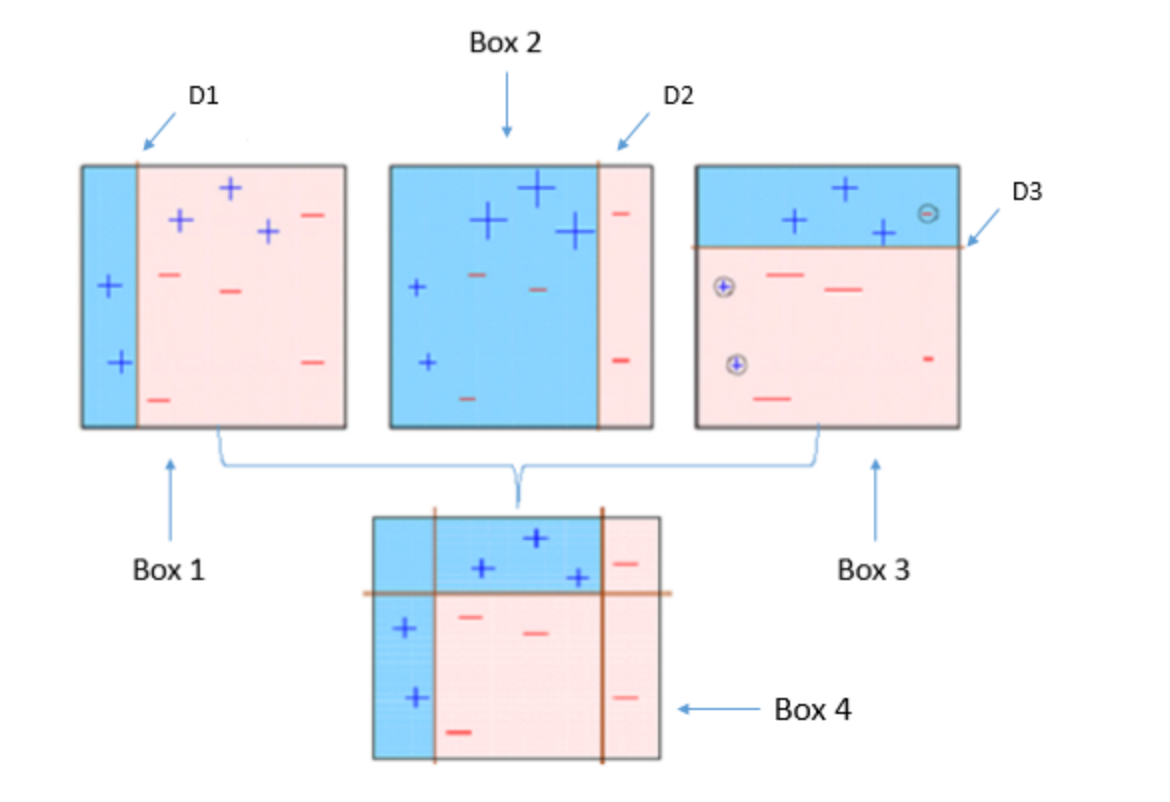
\includegraphics[scale=0.5]{figures/adaboost.png}
              \\
              \tiny
              Source: \url{https://www.analyticsvidhya.com/blog/2015/11/quick-introduction-boosting-algorithms-machine-learning/}
 \end{figure}

\end{frame}
%----------------------------------------------------------------------%
\section{Review
 \& Next Steps}
%----------------------------------------------------------------------%
\begin{frame}
\frametitle{Review \& Next Steps}
  
\begin{itemize} 
   \item Recap w. Example: Beauty in the classroom
   \bigskip
   \item Bagging and Random Forests
   \bigskip
  \item Boosting AdaBoost
    \bigskip  
  \item  Next class:  More on trees, and causal inference


\bigskip  
\item Questions? Questions about software? 

\end{itemize}
\end{frame}
%----------------------------------------------------------------------%
\section{Further Readings}
%----------------------------------------------------------------------%
\begin{frame}
\frametitle{Further Readings}

\begin{itemize}


  \item Breiman, L. (2001). “Random Forests”. In: Machine Learning. ISSN: 1098-6596. DOI: 10.1017/CBO9781107415324.004. eprint: arXiv:1011.1669v3.
  \item Friedman, J., Hastie, T., \& Tibshirani, R. (2001). The elements of statistical learning (Vol. 1, No. 10). New York: Springer series in statistics.
  \medskip
  \item James, G., Witten, D., Hastie, T., \& Tibshirani, R. (2013). An introduction to statistical learning (Vol. 112, p. 18). New York: springer.
  \medskip 
  \item Kasy M. (2019). Trees, forests, and causal trees. Mimeo.
  \medskip
  \item Taddy, M. (2019). Business data science: Combining machine learning and economics to optimize, automate, and accelerate business decisions. McGraw Hill Professional.
  
  
\end{itemize}

\end{frame}






%----------------------------------------------------------------------%
%----------------------------------------------------------------------%
\end{document}
%----------------------------------------------------------------------%
%----------------------------------------------------------------------%

